\documentclass[11pt,]{article}
\usepackage{lmodern}
\usepackage{amssymb,amsmath}
\usepackage{ifxetex,ifluatex}
\usepackage{fixltx2e} % provides \textsubscript
\ifnum 0\ifxetex 1\fi\ifluatex 1\fi=0 % if pdftex
  \usepackage[T1]{fontenc}
  \usepackage[utf8]{inputenc}
\else % if luatex or xelatex
  \ifxetex
    \usepackage{mathspec}
  \else
    \usepackage{fontspec}
  \fi
  \defaultfontfeatures{Ligatures=TeX,Scale=MatchLowercase}
\fi
% use upquote if available, for straight quotes in verbatim environments
\IfFileExists{upquote.sty}{\usepackage{upquote}}{}
% use microtype if available
\IfFileExists{microtype.sty}{%
\usepackage{microtype}
\UseMicrotypeSet[protrusion]{basicmath} % disable protrusion for tt fonts
}{}
\usepackage[margin=1in]{geometry}
\usepackage{hyperref}
\hypersetup{unicode=true,
            pdftitle={Social Equity of Clean Energy Policies on Residential Solar in Seattle},
            pdfauthor={Yohan Min},
            pdfborder={0 0 0},
            breaklinks=true}
\urlstyle{same}  % don't use monospace font for urls
\usepackage{longtable,booktabs}
\usepackage{graphicx,grffile}
\makeatletter
\def\maxwidth{\ifdim\Gin@nat@width>\linewidth\linewidth\else\Gin@nat@width\fi}
\def\maxheight{\ifdim\Gin@nat@height>\textheight\textheight\else\Gin@nat@height\fi}
\makeatother
% Scale images if necessary, so that they will not overflow the page
% margins by default, and it is still possible to overwrite the defaults
% using explicit options in \includegraphics[width, height, ...]{}
\setkeys{Gin}{width=\maxwidth,height=\maxheight,keepaspectratio}
\IfFileExists{parskip.sty}{%
\usepackage{parskip}
}{% else
\setlength{\parindent}{0pt}
\setlength{\parskip}{6pt plus 2pt minus 1pt}
}
\setlength{\emergencystretch}{3em}  % prevent overfull lines
\providecommand{\tightlist}{%
  \setlength{\itemsep}{0pt}\setlength{\parskip}{0pt}}
\setcounter{secnumdepth}{0}
% Redefines (sub)paragraphs to behave more like sections
\ifx\paragraph\undefined\else
\let\oldparagraph\paragraph
\renewcommand{\paragraph}[1]{\oldparagraph{#1}\mbox{}}
\fi
\ifx\subparagraph\undefined\else
\let\oldsubparagraph\subparagraph
\renewcommand{\subparagraph}[1]{\oldsubparagraph{#1}\mbox{}}
\fi

%%% Use protect on footnotes to avoid problems with footnotes in titles
\let\rmarkdownfootnote\footnote%
\def\footnote{\protect\rmarkdownfootnote}

%%% Change title format to be more compact
\usepackage{titling}

% Create subtitle command for use in maketitle
\newcommand{\subtitle}[1]{
  \posttitle{
    \begin{center}\large#1\end{center}
    }
}

\setlength{\droptitle}{-2em}

  \title{Social Equity of Clean Energy Policies on Residential Solar in Seattle}
    \pretitle{\vspace{\droptitle}\centering\huge}
  \posttitle{\par}
    \author{Yohan Min}
    \preauthor{\centering\large\emph}
  \postauthor{\par}
      \predate{\centering\large\emph}
  \postdate{\par}
    \date{Tue Jun 04 15:35:15 2019}

\usepackage{fontspec}
\usepackage{float}
\floatplacement{figure}{H}

\begin{document}
\maketitle

\fontfamily{cmr}
\fontsize{11}{16}
\fontseries{b}
\selectfont

\hypertarget{introduction}{%
\section{1. INTRODUCTION}\label{introduction}}

Residential solar installations have rapidly increased in recent years
with advancement of clean energy policies and associated incentives such
as tax credits. This transition to the new energy system could lead to
undesirable effects on some communities as shown in the case of
telecommunication (Caperton et al.~2013). Committed leadership to
implement a new policy in regard to the transition is required to avoid
the uneven distribution of the service. While numerous studies have been
performed on various aspects of the policies designed to support solar
installations, there is still a dearth of studies aimed at investigating
the impact of such policies on the social equity. Two unanswered
questions have emerged: (1) were there certain communities inadvertently
left out from incentive opportunities? and (2) do those current policies
help the social equity?

To answer these questions, the present study performs a spatial analysis
of the distribution of solar panel installed-buildings (residential
solar hereafter) in terms of housing and socioeconomic characteristics
based on census track in Seattle. In particular, this study aims to
explore any patterns of residential (single family and multifamily)
solar installations by examining spatial clustering patterns,
associations among variables through several data sources.

\hypertarget{data-description}{%
\section{2. DATA DESCRIPTION}\label{data-description}}

City of Seattle open data portal keeps the records of electrical permits
and this study focuses on the data that were issued between 2003 and
2018 in Seattle, WA. Electrical permits are required when residential
houses want to install solar systems on their house properties.
Intensive data mining techniques made it possible to identify
residential solar installation permits among the data sets. The data
includes geographical coordinates (latitude and longitude), completion
of installation dates of the solar system, and solar contractor who
installed the system. Mapping the points of residential solar in the
region can verify a certain pattern in installation. Residential housing
units can be assumed to be evenly present across the region for the
purpose of exploratory data analysis although they are not equally
distributed. The density of point data of residential solar and its
related \texttt{G\ estimate} show a clustered pattern.

\begin{figure}

{\centering 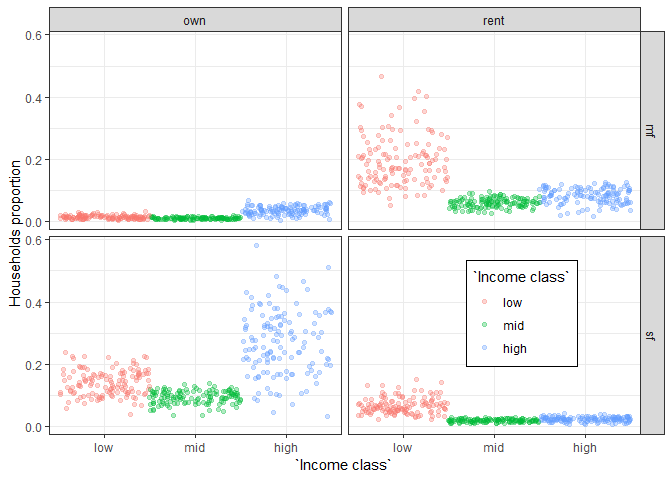
\includegraphics{stat_files/figure-latex/unnamed-chunk-3-1} 

}

\caption{G estimate for spatial dependency of solar installations}\label{fig:unnamed-chunk-3}
\end{figure}

\begin{figure}
\centering
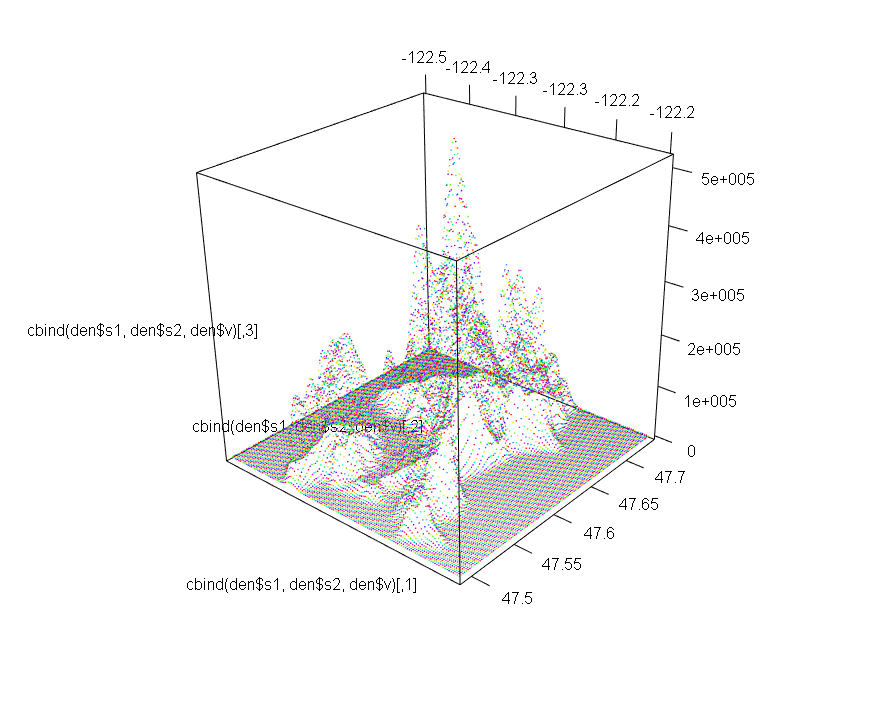
\includegraphics[width=5.20833in,height=\textheight]{3d.png}
\caption{Density plot of residential solar installations in Seattle}
\end{figure}

\begin{figure}

{\centering 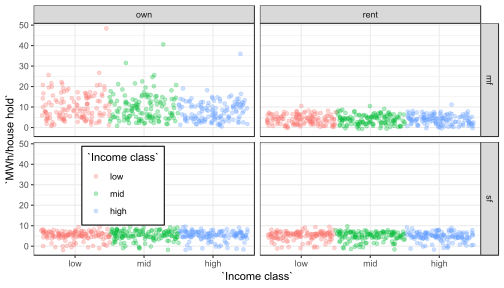
\includegraphics{stat_files/figure-latex/unnamed-chunk-6-1} 

}

\caption{Residential housing density in Seattle}\label{fig:unnamed-chunk-6}
\end{figure}

After the point data was aggregated to the related census track, the
data was examined in terms of the socioeconomic and housing
characteristics based on the American Community Survey of the census
(2011 - 2015 ACS 5-Year estimates). The rate of the residential solar
installation in each census track is the dependent variable
(\texttt{SMR\_s}) in this study. Rest of variables are as follows.

\begin{itemize}
\tightlist
\item
  \texttt{hu\_own}: owner-occupied housing units
\item
  \texttt{single\_unit}: single unit housings (single family houses)
\item
  \texttt{hu\_no\_mor}: owner-occupied housing units without a mortgage
\item
  \texttt{hu\_med\_val}: median value of owner-occupied housing units
\item
  \texttt{edu}: population above high school degree
\item
  \texttt{hh\_med\_income}: household median income
\item
  \texttt{hh\_gini\_index}: household GINI Index of income inequality
\item
  \texttt{high\_income}: high income households
\item
  \texttt{SMR\_s}: the ratio of solar installation to the expected
  number of installations in regard to the total number of the
  residential housing units of the given census track.
\end{itemize}

\begin{figure}

{\centering 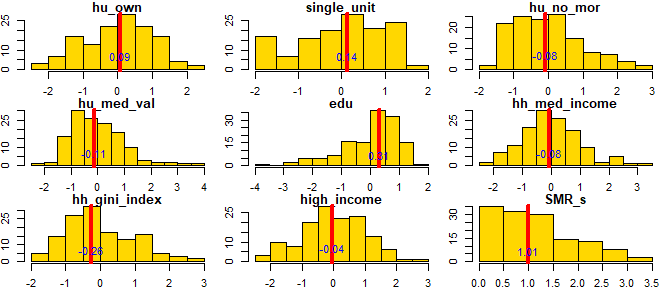
\includegraphics{stat_files/figure-latex/unnamed-chunk-7-1} 

}

\caption{Histograms of variables}\label{fig:unnamed-chunk-7}
\end{figure}

\hypertarget{methods}{%
\section{3. METHODS}\label{methods}}

The expected rate of residential solar per each census track is
estimated based on the total number of housing units in Seattle and its
residential solar numbers. Here the term, Standardized Mortality Ratio
(SMR) can be considered to be the rate of residential solar in a census
track in this study. It is defined by the number of residential solar
over the expected number of residential solar given the estimated
proportion, which is the total number of residential solar over the
total number of housing units in Seattle. SMR shows a pattern of
clustering similar to the pattern of the previous point data of
residential solar.

\[ SMR_i = \frac{Y_i}{E_i} \]

The residential solar rate is assumed to be associated with
\texttt{poisson\ count\ model} considering its rare proportion with
respect to the denominator (the total housing units) in a census track
in addition to the fact that the number of residential solar is count
data. The residuals, after fitting the poisson model, shows clustering
with the similar pattern of SMR distribution across census tracks as
shown in the figures below. This indicates that there is strong evidence
of spatial dependency among the regions in Seattle. \[
\begin{aligned}
Y_i \sim \mbox{Poisson}(E_i \mbox{e}^{\beta_{0}})
\end{aligned}
\]

\begin{figure}

{\centering 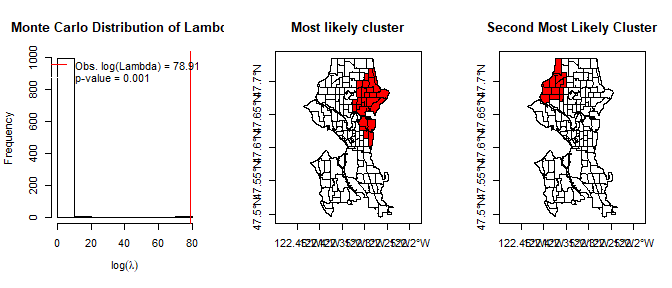
\includegraphics{stat_files/figure-latex/unnamed-chunk-9-1} 

}

\caption{SMR and residuals of poisson model}\label{fig:unnamed-chunk-9}
\end{figure}

Moran's I test detects global clustering in the distribution of the rate
of residential solar with very small \texttt{p-value}. This confirms
that the residential solar rate across census tracks is clustered. Using
\texttt{SatScan\ method}, area clustering detection shows Northwest
Seattle and Northeast Seattle as the clustered regions. This clustering
trend can be alleviated by fitting a model with appropriate covariates
showing the similar characteristics. In this regard, socioeconomic and
housing characteristics will be examined to identify the most proper
covariates.

\begin{figure}

{\centering 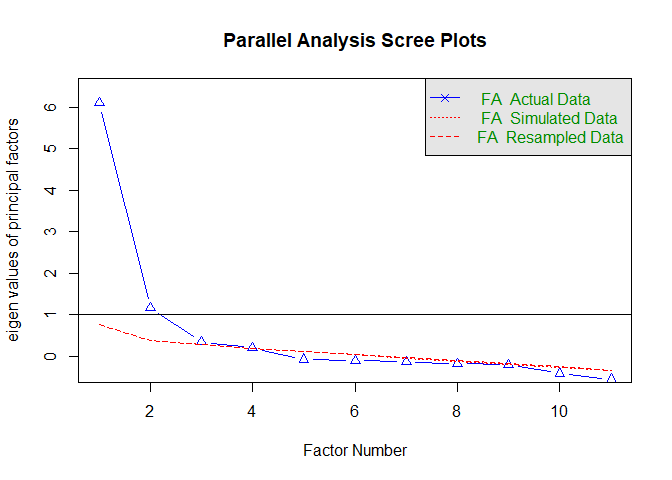
\includegraphics{stat_files/figure-latex/unnamed-chunk-10-1} 

}

\caption{StaScan clustering detection}\label{fig:unnamed-chunk-10}
\end{figure}

Having verified that there is a spatial pattern in the residential solar
rate, there might be related or shared factors in socioeconomic and
housing characteristics in the same region. Housing, economy, social
inequality variables show correlations pairwise in the figure below.

\begin{figure}

{\centering 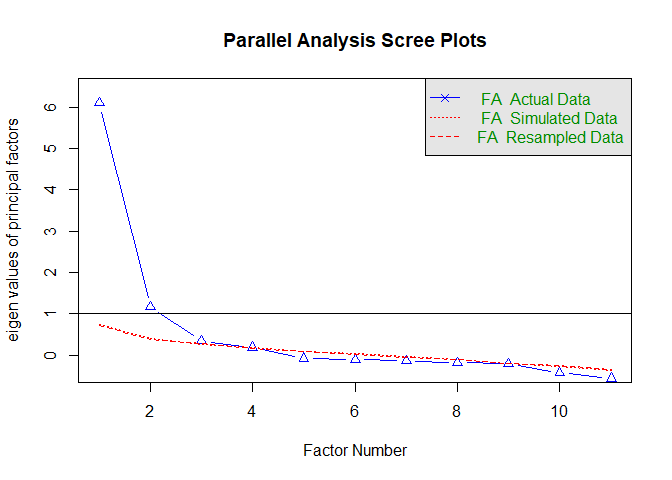
\includegraphics{stat_files/figure-latex/unnamed-chunk-11-1} 

}

\caption{Covariates correlation plot}\label{fig:unnamed-chunk-11}
\end{figure}

Dimension reduction of covariates will be performed by factor analysis
in consideration of avoiding multicollinearity. The newly generated
factors will fit models to estimate the residential solar rate.
Residuals will be checked afterwards to see if there is still a
clustering pattern, which indicates that the model can't address the
spatial dependency. Furthermore, a few variables which represent each
factor the most, will be chosen for the model fit compared to the
factors from dimension reduction. It is because factors could possibly
keep overall noises by including unnecessary covariates, which are less
related to the residential solar rate. Poisson lognormal spatial model,
specially using \texttt{BYM2} method, will be tested to address the
residual clustering issue in addition to \texttt{K-means} clustering
analysis, which identifies similar regions in terms of socioeconomic and
housing patterns of census tracks. Note that \texttt{K-means} clustering
will not take into account of the residential solar rate for defining
the Euclidean distance among data points in order for the categorized
census tracks to be compared with the residential solar rate pattern to
figure out the relationship between the covariates and residential solar
rate. Finally Geographically Weighted Regression (GWR) will address the
local variation of coefficients of covariates by taking into account of
the local spatial dependency.

\hypertarget{results}{%
\section{4. RESULTS}\label{results}}

\hypertarget{factor-analysis}{%
\subsection{4.1. Factor analysis}\label{factor-analysis}}

Factor analysis was performed to reduce dimension of variables in
accordance with variables representing similar characteristics, mostly
correlated each other. It identifies the similar variables in terms of
housing unit structure (single/ multi-family house unit), housing tenure
(rent/ owns), economic status (income level and housing value), and
inequality index. Housing unit structure shows the similar trend of
housing tenure while housing median value, high income class proportion,
and household median income follow the similar pattern representing
economic status. Residential solar rate and the factors from the
dimension reduction, show strong correlations. Generalized log-linear
model was fitted to the data.

\begin{figure}

{\centering 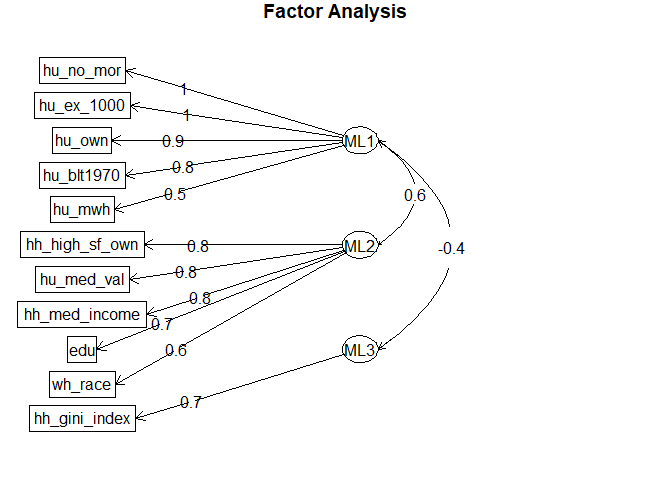
\includegraphics{stat_files/figure-latex/unnamed-chunk-13-1} 

}

\caption{Factor diagram}\label{fig:unnamed-chunk-13}
\end{figure}

\begin{longtable}[]{@{}ccccc@{}}
\caption{Fitting generalized (poisson/log) linear model: n\_s
\textasciitilde{} ML1 + ML2 + offset(log(solar\_E))}\tabularnewline
\toprule
\begin{minipage}[b]{0.21\columnwidth}\centering
~\strut
\end{minipage} & \begin{minipage}[b]{0.13\columnwidth}\centering
Estimate\strut
\end{minipage} & \begin{minipage}[b]{0.16\columnwidth}\centering
Std. Error\strut
\end{minipage} & \begin{minipage}[b]{0.12\columnwidth}\centering
z value\strut
\end{minipage} & \begin{minipage}[b]{0.16\columnwidth}\centering
Pr(\textgreater{}\textbar{}z\textbar{})\strut
\end{minipage}\tabularnewline
\midrule
\endfirsthead
\toprule
\begin{minipage}[b]{0.21\columnwidth}\centering
~\strut
\end{minipage} & \begin{minipage}[b]{0.13\columnwidth}\centering
Estimate\strut
\end{minipage} & \begin{minipage}[b]{0.16\columnwidth}\centering
Std. Error\strut
\end{minipage} & \begin{minipage}[b]{0.12\columnwidth}\centering
z value\strut
\end{minipage} & \begin{minipage}[b]{0.16\columnwidth}\centering
Pr(\textgreater{}\textbar{}z\textbar{})\strut
\end{minipage}\tabularnewline
\midrule
\endhead
\begin{minipage}[t]{0.21\columnwidth}\centering
\textbf{(Intercept)}\strut
\end{minipage} & \begin{minipage}[t]{0.13\columnwidth}\centering
-0.1107\strut
\end{minipage} & \begin{minipage}[t]{0.16\columnwidth}\centering
0.02038\strut
\end{minipage} & \begin{minipage}[t]{0.12\columnwidth}\centering
-5.432\strut
\end{minipage} & \begin{minipage}[t]{0.16\columnwidth}\centering
5.588e-08\strut
\end{minipage}\tabularnewline
\begin{minipage}[t]{0.21\columnwidth}\centering
\textbf{ML1}\strut
\end{minipage} & \begin{minipage}[t]{0.13\columnwidth}\centering
0.5678\strut
\end{minipage} & \begin{minipage}[t]{0.16\columnwidth}\centering
0.02233\strut
\end{minipage} & \begin{minipage}[t]{0.12\columnwidth}\centering
25.43\strut
\end{minipage} & \begin{minipage}[t]{0.16\columnwidth}\centering
1.132e-142\strut
\end{minipage}\tabularnewline
\begin{minipage}[t]{0.21\columnwidth}\centering
\textbf{ML2}\strut
\end{minipage} & \begin{minipage}[t]{0.13\columnwidth}\centering
0.1451\strut
\end{minipage} & \begin{minipage}[t]{0.16\columnwidth}\centering
0.0216\strut
\end{minipage} & \begin{minipage}[t]{0.12\columnwidth}\centering
6.718\strut
\end{minipage} & \begin{minipage}[t]{0.16\columnwidth}\centering
1.843e-11\strut
\end{minipage}\tabularnewline
\bottomrule
\end{longtable}

\begin{figure}

{\centering 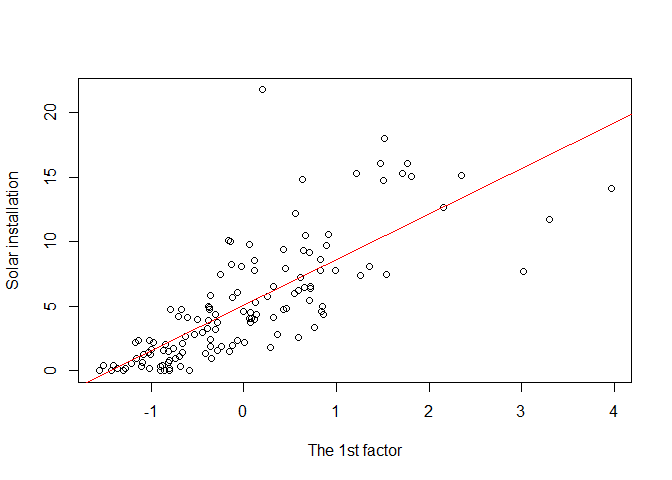
\includegraphics{stat_files/figure-latex/unnamed-chunk-14-1} 

}

\caption{SMR plots in factors}\label{fig:unnamed-chunk-14}
\end{figure}

\hypertarget{integrated-nested-laplace-approximations-inla-model}{%
\subsection{4.2. Integrated Nested Laplace Approximations (INLA)
model}\label{integrated-nested-laplace-approximations-inla-model}}

It is obvious that the variables can be divided into three categories:
(1) housing stability, mostly the proportion of owner occupied single
family houses, (2) economic status such as income level and house value,
and (3) income inequality. Solar installation rate seems to be mainly
correlated to the housing stability and economic status in this data. A
few selected covariates could fit a model better than factors due to the
fact that factors include all the unrelated covariates to the dependent
variable (residential solar rate) in this study. The most representing
covariates are single family house proportion (housing stability) and
house median value (economic status) and selected for the further
analyses. It is verified that the same generalized loglinear model fits
better with the two covariates than factors.

\[
\begin{aligned}
Y_i |\beta_{0},\beta_{1},\beta_{2},S_i,\epsilon_i & \sim_{ind} \mbox{Poisson}(E_i \mbox{e}^{\beta_{0}+\beta_{1}I_{1i}+\beta_{2}I_{2i}} \mbox{e}^{S_i + \epsilon_i}),\\ 
\epsilon_i | \sigma_\epsilon^{2} & \sim_{iid} \mbox{N}(0,\sigma_\epsilon^{2}),\\ 
S_1,...,S_n | \sigma_s^{2} & \sim ~~~ \mbox{ICAR}(\sigma_s^{2}). 
\end{aligned} 
\]

Integrated Nested Laplace Approximations (INLA) model takes into account
of spatial dependencies and lognormal independent variance across census
tracks. This model was set with priors such that 50\% chance that the
proportion of the spatial variance, \(\phi\) is greater 0.5 and 1\%
chance that the total residual standard deviation is greater than 0.9.
The result of the model fit confirms that the large variance is due to
the spatial factor with \(\phi\) of 0.96 in median.

\begin{longtable}[]{@{}ccccc@{}}
\caption{Fitting INLA model: n\_s \textasciitilde{}
offset(log(solar\_E)) + ML1 + ML2}\tabularnewline
\toprule
\begin{minipage}[b]{0.29\columnwidth}\centering
~\strut
\end{minipage} & \begin{minipage}[b]{0.12\columnwidth}\centering
mean\strut
\end{minipage} & \begin{minipage}[b]{0.16\columnwidth}\centering
0.025quant\strut
\end{minipage} & \begin{minipage}[b]{0.13\columnwidth}\centering
0.5quant\strut
\end{minipage} & \begin{minipage}[b]{0.16\columnwidth}\centering
0.975quant\strut
\end{minipage}\tabularnewline
\midrule
\endfirsthead
\toprule
\begin{minipage}[b]{0.29\columnwidth}\centering
~\strut
\end{minipage} & \begin{minipage}[b]{0.12\columnwidth}\centering
mean\strut
\end{minipage} & \begin{minipage}[b]{0.16\columnwidth}\centering
0.025quant\strut
\end{minipage} & \begin{minipage}[b]{0.13\columnwidth}\centering
0.5quant\strut
\end{minipage} & \begin{minipage}[b]{0.16\columnwidth}\centering
0.975quant\strut
\end{minipage}\tabularnewline
\midrule
\endhead
\begin{minipage}[t]{0.29\columnwidth}\centering
\textbf{(Intercept)}\strut
\end{minipage} & \begin{minipage}[t]{0.12\columnwidth}\centering
-0.3031\strut
\end{minipage} & \begin{minipage}[t]{0.16\columnwidth}\centering
-0.3624\strut
\end{minipage} & \begin{minipage}[t]{0.13\columnwidth}\centering
-0.3028\strut
\end{minipage} & \begin{minipage}[t]{0.16\columnwidth}\centering
-0.2455\strut
\end{minipage}\tabularnewline
\begin{minipage}[t]{0.29\columnwidth}\centering
\textbf{I(ML1)}\strut
\end{minipage} & \begin{minipage}[t]{0.12\columnwidth}\centering
0.5549\strut
\end{minipage} & \begin{minipage}[t]{0.16\columnwidth}\centering
0.4107\strut
\end{minipage} & \begin{minipage}[t]{0.13\columnwidth}\centering
0.5548\strut
\end{minipage} & \begin{minipage}[t]{0.16\columnwidth}\centering
0.6995\strut
\end{minipage}\tabularnewline
\begin{minipage}[t]{0.29\columnwidth}\centering
\textbf{I(ML2)}\strut
\end{minipage} & \begin{minipage}[t]{0.12\columnwidth}\centering
0.182\strut
\end{minipage} & \begin{minipage}[t]{0.16\columnwidth}\centering
0.0429\strut
\end{minipage} & \begin{minipage}[t]{0.13\columnwidth}\centering
0.1816\strut
\end{minipage} & \begin{minipage}[t]{0.16\columnwidth}\centering
0.3232\strut
\end{minipage}\tabularnewline
\begin{minipage}[t]{0.29\columnwidth}\centering
\textbf{Total residual sd}\strut
\end{minipage} & \begin{minipage}[t]{0.12\columnwidth}\centering
0.662\strut
\end{minipage} & \begin{minipage}[t]{0.16\columnwidth}\centering
0.8032\strut
\end{minipage} & \begin{minipage}[t]{0.13\columnwidth}\centering
0.6676\strut
\end{minipage} & \begin{minipage}[t]{0.16\columnwidth}\centering
0.5564\strut
\end{minipage}\tabularnewline
\begin{minipage}[t]{0.29\columnwidth}\centering
\textbf{Phi for ID}\strut
\end{minipage} & \begin{minipage}[t]{0.12\columnwidth}\centering
0.9611\strut
\end{minipage} & \begin{minipage}[t]{0.16\columnwidth}\centering
0.8347\strut
\end{minipage} & \begin{minipage}[t]{0.13\columnwidth}\centering
0.9765\strut
\end{minipage} & \begin{minipage}[t]{0.16\columnwidth}\centering
0.9988\strut
\end{minipage}\tabularnewline
\bottomrule
\end{longtable}

Even though this model considers the spatial dependency, the residuals
for the model show a clustering pattern after eliminating the covariate
terms from the fitted values.

\hypertarget{k-means-clustering-analysis}{%
\subsection{4.3. K-means clustering
analysis}\label{k-means-clustering-analysis}}

K-means cluster analysis indicates a group of census tracks with the
similar characteristics which helps to identify the correlations between
concerned covariates and the dependent variable (residential solar
rate). Three groups are categorized with the census tracks in Seattle.
The clustering pattern is evident with respect to the covariates, house
median value and the proportion of single family house units.

\begin{figure}

{\centering 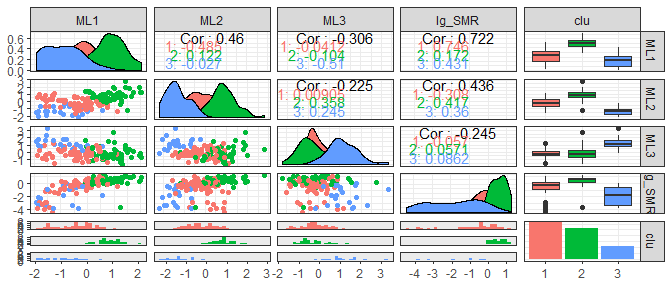
\includegraphics{stat_files/figure-latex/unnamed-chunk-18-1} 

}

\caption{Covariate distributions with clustering}\label{fig:unnamed-chunk-18}
\end{figure}

\hypertarget{geographically-weighted-regression}{%
\subsection{4.4. Geographically Weighted
Regression}\label{geographically-weighted-regression}}

Geographically Weighted Regression (GWR) model finally confirms that the
residuals of the model have less chance of spatial dependency with
respect to the insignificant \texttt{p-value} of Moran's I in 0.05
significance level. This model has even higher \texttt{R-squared} value
compared to the previous models. GWR model entails consideration of
spatial dependence in a local level by changing the coefficient values
of covariates without involvement of explicit spatial term to the model.
Below figures show the variance of coefficient values across the census
tracks. The intensity of each map of covariates indicates the
sensitivity of the concerned covariate in terms of the rate of
residential solar. Single family house rate impacts more on the central
Seattle area while North and South Seattle are more sensitive to the
house median value with respect to solar panel installation on the
residential houses.

\[
\begin{aligned}
Y(s) = E(s)\mbox{e}^{(\beta_{0}+\beta_{1}(s)X_1(s)+\beta_{2}(s)X_2(s)+\epsilon(s))}
\end{aligned} 
\]

\begin{figure}

{\centering 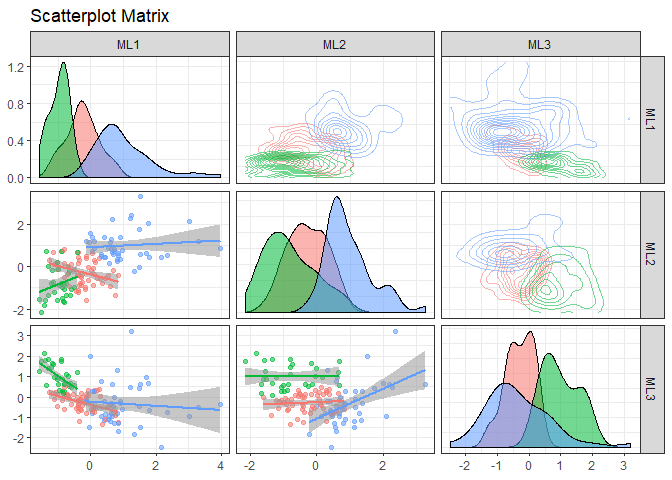
\includegraphics{stat_files/figure-latex/unnamed-chunk-22-1} 

}

\caption{Clustering and GWR residuals}\label{fig:unnamed-chunk-22}
\end{figure}
\begin{figure}

{\centering 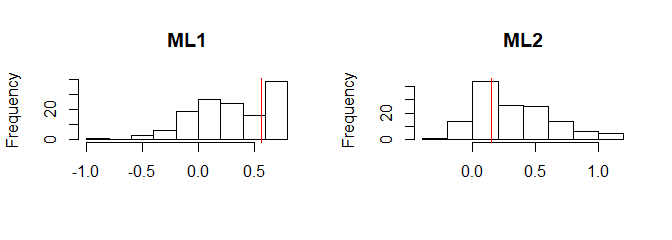
\includegraphics{stat_files/figure-latex/unnamed-chunk-23-1} 

}

\caption{Coefficient variation of covariates}\label{fig:unnamed-chunk-23}
\end{figure}
\begin{figure}

{\centering 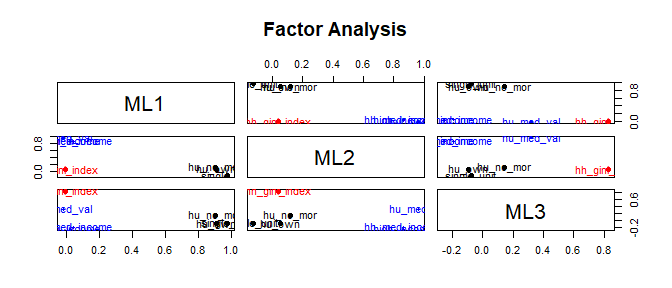
\includegraphics{stat_files/figure-latex/unnamed-chunk-24-1} 

}

\caption{GWR different impact of covariates in Seattle}\label{fig:unnamed-chunk-24}
\end{figure}

\hypertarget{discussion-and-conclusion}{%
\section{5. DISCUSSION AND CONCLUSION}\label{discussion-and-conclusion}}

The previous analyses reveal that (1) residential solar installations
are mostly correlated to housing stability (single family house unit and
housing tenure) and economic status (income level and house value) (2)
income inequality across census tracks is less likely correlated. The
results answer the questions that there are certain communities left out
from using renewable energy due to the lack of resources (i.e., housing
and finance). Since these communities are hard to join the incentivized
programs such as 30\% federal tax credits, it is necessary to address
the issue by coming up with policies such that encouraging the
underserved communities to take advantage of the clean energy as well.
In addition, cluster and GWR model with respect to the residential solar
were analyzed to find areas in Seattle more influenced by each
characteristic. As a result, three categorized groups in terms of
housing stability and economic status were identified in addition to
areas in Seattle where residential solar installations are more
sensitive to the economic status and the housing stability.

The study results will support policy makers to develop a policy that
better help underserved communities under limited resources (e.g., those
who rent multi-family houses and have less finance to install solar
systems) by leading to equitable incentive distribution and access to
clean energy.

\hypertarget{reference}{%
\section{REFERENCE}\label{reference}}

Caperton, Richard W., Mari Hern, and ez. ``The Electrical Divide: New
Energy Technologies and Avoiding an Electric Service Gap.'' Center for
American Progress. Accessed December 24, 2018.
\url{https://www.americanprogress.org/issues/green/reports/2013/07/15/69249/the-electrical-divide-new-energy-technologies-and-avoiding-an-electric-service-gap/}.

\pagebreak

\hypertarget{appendix}{%
\section{APPENDIX}\label{appendix}}

\begin{longtable}[]{@{}cccc@{}}
\caption{Residuals of poisson model without covariates (continued
below)}\tabularnewline
\toprule
\begin{minipage}[b]{0.19\columnwidth}\centering
Test statistic\strut
\end{minipage} & \begin{minipage}[b]{0.20\columnwidth}\centering
P value\strut
\end{minipage} & \begin{minipage}[b]{0.28\columnwidth}\centering
Alternative hypothesis\strut
\end{minipage} & \begin{minipage}[b]{0.22\columnwidth}\centering
Moran I statistic\strut
\end{minipage}\tabularnewline
\midrule
\endfirsthead
\toprule
\begin{minipage}[b]{0.19\columnwidth}\centering
Test statistic\strut
\end{minipage} & \begin{minipage}[b]{0.20\columnwidth}\centering
P value\strut
\end{minipage} & \begin{minipage}[b]{0.28\columnwidth}\centering
Alternative hypothesis\strut
\end{minipage} & \begin{minipage}[b]{0.22\columnwidth}\centering
Moran I statistic\strut
\end{minipage}\tabularnewline
\midrule
\endhead
\begin{minipage}[t]{0.19\columnwidth}\centering
8.809\strut
\end{minipage} & \begin{minipage}[t]{0.20\columnwidth}\centering
6.327e-19 * * *\strut
\end{minipage} & \begin{minipage}[t]{0.28\columnwidth}\centering
greater\strut
\end{minipage} & \begin{minipage}[t]{0.22\columnwidth}\centering
0.4706\strut
\end{minipage}\tabularnewline
\bottomrule
\end{longtable}

\begin{longtable}[]{@{}cc@{}}
\toprule
\begin{minipage}[b]{0.18\columnwidth}\centering
Expectation\strut
\end{minipage} & \begin{minipage}[b]{0.14\columnwidth}\centering
Variance\strut
\end{minipage}\tabularnewline
\midrule
\endhead
\begin{minipage}[t]{0.18\columnwidth}\centering
-0.007463\strut
\end{minipage} & \begin{minipage}[t]{0.14\columnwidth}\centering
0.002945\strut
\end{minipage}\tabularnewline
\bottomrule
\end{longtable}

\begin{longtable}[]{@{}cccc@{}}
\caption{Residuals of poission model with covariates (continued
below)}\tabularnewline
\toprule
\begin{minipage}[b]{0.19\columnwidth}\centering
Test statistic\strut
\end{minipage} & \begin{minipage}[b]{0.20\columnwidth}\centering
P value\strut
\end{minipage} & \begin{minipage}[b]{0.28\columnwidth}\centering
Alternative hypothesis\strut
\end{minipage} & \begin{minipage}[b]{0.22\columnwidth}\centering
Moran I statistic\strut
\end{minipage}\tabularnewline
\midrule
\endfirsthead
\toprule
\begin{minipage}[b]{0.19\columnwidth}\centering
Test statistic\strut
\end{minipage} & \begin{minipage}[b]{0.20\columnwidth}\centering
P value\strut
\end{minipage} & \begin{minipage}[b]{0.28\columnwidth}\centering
Alternative hypothesis\strut
\end{minipage} & \begin{minipage}[b]{0.22\columnwidth}\centering
Moran I statistic\strut
\end{minipage}\tabularnewline
\midrule
\endhead
\begin{minipage}[t]{0.19\columnwidth}\centering
7.214\strut
\end{minipage} & \begin{minipage}[t]{0.20\columnwidth}\centering
2.725e-13 * * *\strut
\end{minipage} & \begin{minipage}[t]{0.28\columnwidth}\centering
greater\strut
\end{minipage} & \begin{minipage}[t]{0.22\columnwidth}\centering
0.3811\strut
\end{minipage}\tabularnewline
\bottomrule
\end{longtable}

\begin{longtable}[]{@{}cc@{}}
\toprule
\begin{minipage}[b]{0.18\columnwidth}\centering
Expectation\strut
\end{minipage} & \begin{minipage}[b]{0.14\columnwidth}\centering
Variance\strut
\end{minipage}\tabularnewline
\midrule
\endhead
\begin{minipage}[t]{0.18\columnwidth}\centering
-0.007463\strut
\end{minipage} & \begin{minipage}[t]{0.14\columnwidth}\centering
0.002902\strut
\end{minipage}\tabularnewline
\bottomrule
\end{longtable}

\begin{figure}

{\centering 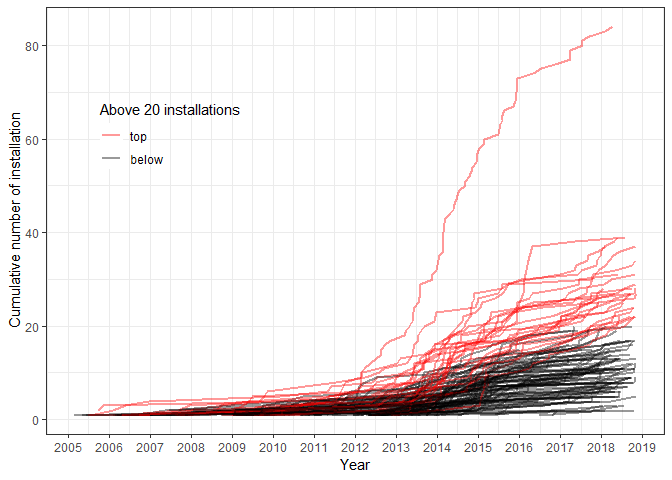
\includegraphics{stat_files/figure-latex/unnamed-chunk-25-1} 

}

\caption{Factors in tersm of covariates}\label{fig:unnamed-chunk-25}
\end{figure}
\begin{figure}

{\centering 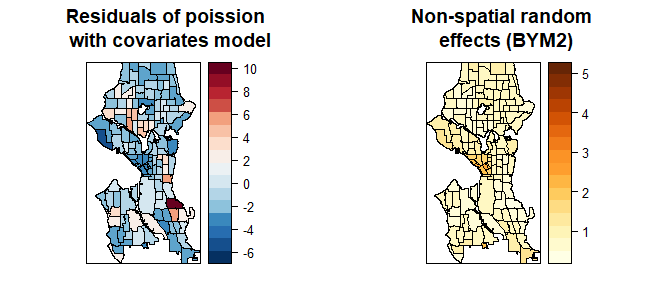
\includegraphics{stat_files/figure-latex/unnamed-chunk-26-1} 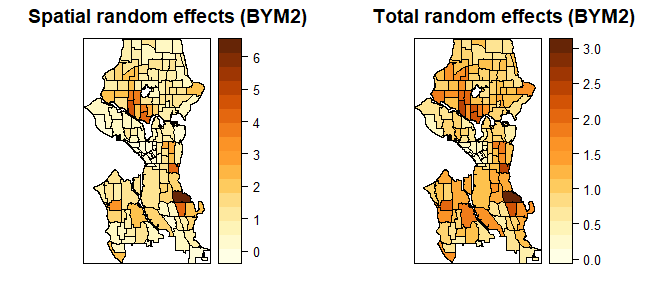
\includegraphics{stat_files/figure-latex/unnamed-chunk-26-2} 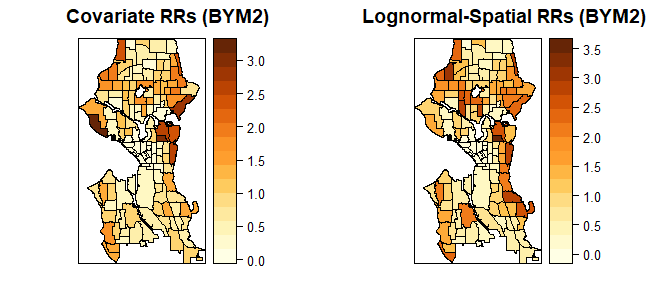
\includegraphics{stat_files/figure-latex/unnamed-chunk-26-3} 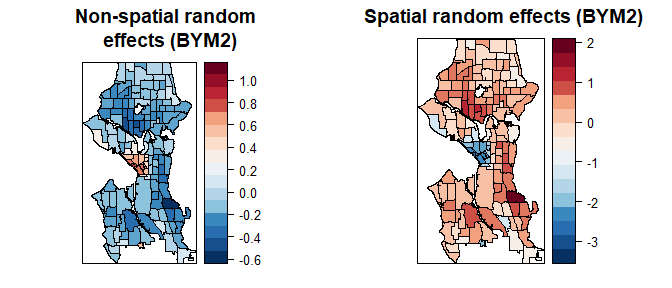
\includegraphics{stat_files/figure-latex/unnamed-chunk-26-4} 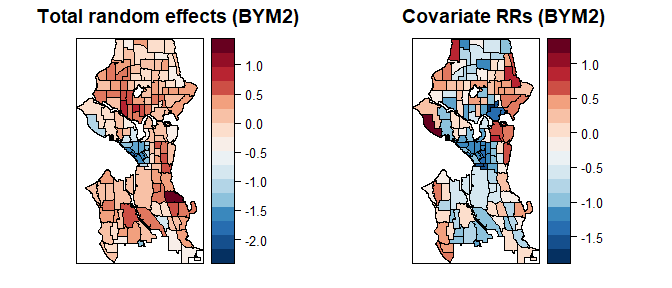
\includegraphics{stat_files/figure-latex/unnamed-chunk-26-5} 

}

\caption{Mapping of random effects and residuals}\label{fig:unnamed-chunk-26}
\end{figure}

\begin{longtable}[]{@{}cccc@{}}
\caption{GWR residual residuals (continued below)}\tabularnewline
\toprule
\begin{minipage}[b]{0.19\columnwidth}\centering
Test statistic\strut
\end{minipage} & \begin{minipage}[b]{0.20\columnwidth}\centering
P value\strut
\end{minipage} & \begin{minipage}[b]{0.28\columnwidth}\centering
Alternative hypothesis\strut
\end{minipage} & \begin{minipage}[b]{0.22\columnwidth}\centering
Moran I statistic\strut
\end{minipage}\tabularnewline
\midrule
\endfirsthead
\toprule
\begin{minipage}[b]{0.19\columnwidth}\centering
Test statistic\strut
\end{minipage} & \begin{minipage}[b]{0.20\columnwidth}\centering
P value\strut
\end{minipage} & \begin{minipage}[b]{0.28\columnwidth}\centering
Alternative hypothesis\strut
\end{minipage} & \begin{minipage}[b]{0.22\columnwidth}\centering
Moran I statistic\strut
\end{minipage}\tabularnewline
\midrule
\endhead
\begin{minipage}[t]{0.19\columnwidth}\centering
3.49\strut
\end{minipage} & \begin{minipage}[t]{0.20\columnwidth}\centering
0.0002416 * * *\strut
\end{minipage} & \begin{minipage}[t]{0.28\columnwidth}\centering
greater\strut
\end{minipage} & \begin{minipage}[t]{0.22\columnwidth}\centering
0.1783\strut
\end{minipage}\tabularnewline
\bottomrule
\end{longtable}

\begin{longtable}[]{@{}cc@{}}
\toprule
\begin{minipage}[b]{0.18\columnwidth}\centering
Expectation\strut
\end{minipage} & \begin{minipage}[b]{0.14\columnwidth}\centering
Variance\strut
\end{minipage}\tabularnewline
\midrule
\endhead
\begin{minipage}[t]{0.18\columnwidth}\centering
-0.007463\strut
\end{minipage} & \begin{minipage}[t]{0.14\columnwidth}\centering
0.002833\strut
\end{minipage}\tabularnewline
\bottomrule
\end{longtable}

\begin{figure}

{\centering 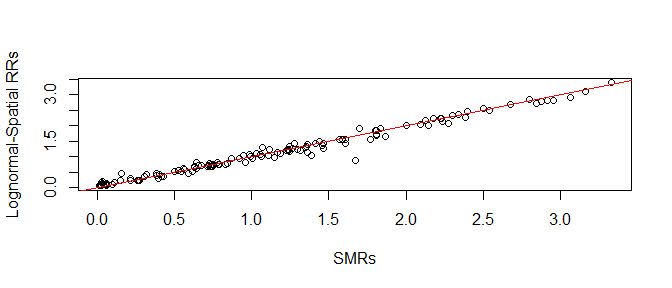
\includegraphics{stat_files/figure-latex/unnamed-chunk-27-1} 

}

\caption{Plot of SMR vs. RR from INLA model}\label{fig:unnamed-chunk-27}
\end{figure}


\end{document}
